\documentclass[a4paper]{article}

\usepackage[spanish]{babel}
\usepackage[utf8]{inputenc}
\usepackage{amsmath}
\usepackage[final]{graphicx}
\usepackage[top=1.25in, bottom=1.25in, left=1in, right=1in]{geometry}
\usepackage[colorinlistoftodos]{todonotes}
\usepackage{minted}
\usepackage{hyperref}
\hypersetup{
    colorlinks=true,
    linkcolor=blue,
    filecolor=magenta,      
    urlcolor=cyan,
    pdftitle={Overleaf Example},
    pdfpagemode=FullScreen,
    }
\urlstyle{same}
\usepackage{listings}
\usepackage{xcolor}

\definecolor{codegreen}{rgb}{0,0.6,0}
\definecolor{codegray}{rgb}{0.5,0.5,0.5}
\definecolor{codepurple}{rgb}{0.58,0,0.82}
\definecolor{backcolour}{rgb}{0.95,0.95,0.92}

\lstdefinestyle{Python}{
    backgroundcolor=\color{backcolour},   
    commentstyle=\color{codegreen},
    keywordstyle=\color{magenta},
    numberstyle=\tiny\color{codegray},
    stringstyle=\color{codepurple},
    basicstyle=\ttfamily\footnotesize,
    breakatwhitespace=false,         
    breaklines=true,                 
    captionpos=b,                    
    keepspaces=true,                 
    numbers=left,                    
    numbersep=5pt,                  
    showspaces=false,                
    showstringspaces=false,
    showtabs=false,                  
    tabsize=2
}

\begin{document}
\begin{center}
\large{PROPUESTAS DE PROYECTO - BIG DATA}\\
\small{Estudiante: Yoksan Varela Cambronero}\\
\small{3 de Julio, 2024}
\end{center}

\section{Investigación preliminar}

\subsection{Primera propuesta: Un nuevo desarrollador de video juegos}
\subsubsection{Problema a resolver}
De acuerdo con el artículo publicado por \textit{Fortune Business Insights} (\url{https://www.fortunebusinessinsights.com/video-game-market-102548}), el valor de mercado de los video juegos era de aproximadamente de \$250 mil millones para 2022, y se espera un crecimiento a una tasa compuesta anual (CAGR por sus siglas en inglés) del 13.1\%, lo que implica que alcanzar\'{a} los \$665 mil millones para 2030.\\

Una nueva desarrolla costarricense de video juegos quiere formar parte de este crecimiento de mercado y obtener una parte de ese dinero. Dicha desarrolladora hizo una inversión importante en todo lo referente a infraestructura para el desarrollo de un nuevo juego, pero pero esto produjo un problema: Para poder recuperar su inversión, los cálculos realizados indican que este nuevo viejo juego tiene que vender m\'{a}s de 100 mil copias, por lo tanto, esta empresa necesita entender cuál es la receta que les permita llegar a esa meta tan agresiva.

\subsubsection{Solución propuesta}
Se le plantea a dicha empresa crea una sistema de aprendizaje automático que pueda predecir si el nuevo video juego va a llegar a vender la cantidad deseada o, en su defecto, no va a alcanzar las 100 mil copias en ventas.

\subsubsection{Fuentes de datos}
Para hacer este estudio de mercado, se van a utilizar dos conjuntos de datos tomados de Kaggle:

\subsubsection{Primer set: Video Games Dataset}
URL: \url{https://www.kaggle.com/datasets/beridzeg45/video-games}\\
    Este conjunto de datos cuenta con información de 14035 video juegos. Los atributos que contiene dicho documento es:
    \begin{enumerate}
        \item \textit{Title:} Nombre del video juego.
        \item \textit{Release Date:} Fecha del lanzamiento del video juego.
        \item \textit{Developer:} Desarrollador del video juego.
        \item \textit{Publisher:} Editor del video juego (quien provee el financiamiento del mismo, incluyendo mercadeo y promoción).
        \item \textit{Genres:} Tipo a cual pertenece el video juego, por ejemplo: acción, aventura, roles, deportes, etc.
        \item \textit{Product Rating:} Es la calificación del producto, en este caso, quienes deber\'{i}n jugar el juego: apto para todo publico, mayores de cierta edad, adultos, etc.
        \item \textit{User Score:} Puntaje de evaluación impuesto por el jugador final.
        \item \textit{User Rating Count:} Conteo de veces que el juego recibió un puntaje por parte de un jugador.
        \item \textit{Platforms info:} Información de las plataformas donde se juega el juego, pero en forma de diccionario.
    \end{enumerate}\newpage

\subsubsection{Calidad de datos:}
Este análisis empieza con entender la cantidad de valores NaN presentes en el conjunto de datos. Los resultados se tabulan a continuación:
    
    \begin{table}[hbtp!]
        \centering
        \begin{tabular}{|c|c|}
            \hline
            \textbf{Atributo} & \textbf{Conteo de NaN}\\
            \hline
            Title & 21\\
            \hline
            Release Date & 64\\
            \hline
            Developer & 138\\
            \hline
            Publisher & 138\\
            \hline
            Genres & 21\\
            \hline
            Product Rating & 3050\\
            \hline
            User Score & 2341\\
            \hline
            User Rating Count & 2756\\
            \hline
            Platforms info & 0\\
            \hline
        \end{tabular}
        \caption{Conteo de valores NaN en el set de datos Video Game Dataset}
        \label{tab:conteo_nan_info_videojuegos}
    \end{table}

    Para lidiar con los valores NaN, se decide reemplazar los NaN en con "Not Specified" en los siguientes atributos: Genres, Publisher y Product Rating, dado que se consideran atributos de interés para el estudio debido a su conocido impacto en las ventas de un video juego. Adem\'{a}s, para el atributo Product Score se decide reemplazar los NaN por el valor medio del atributo, por la misma razón explicada anteriormente.

    Los siguientes atributos fueron descartados por lo siguiente:
    \begin{enumerate}
        \item User Ratings Count: Este conteo carece de información importante, que la vez es redundante con User Score.
        \item Platforms Info: Este atributo se puede obtener del otro set de datos que se explicará posteriormente de una forma más fácil.
        \item Developer: Dado que el cliente es un desarrollador en sí, no esta interesado en saber quién desarrolló el juego para evitar comparaciones con desarrolladores más establecidos y con mayor capital de operación.
    \end{enumerate}

    Ya con estos cambios hecho, se procede a descartar las instancias que tienen NaN en Title y Release Date para obtener el set de datos limpios y proceder a analizar de forma estad\'{i}stica. Al final de estos pasos, quedaron 13991 instancias.

\subsubsection{Análisis del primer set de datos:}
Este conjunto de datos presenta 4752 fechas de lanzamiento distintas, 2302 editores y 119 diferentes tipos de juego. Usar estadística descriptiva en estas categorías representa visuales sumamente difíciles de interpretar, por lo tanto, solo se van a analizar de forma visual el Product Rating y el User Score:\newpage

    \begin{figure}[hbtp!]
        \centering
        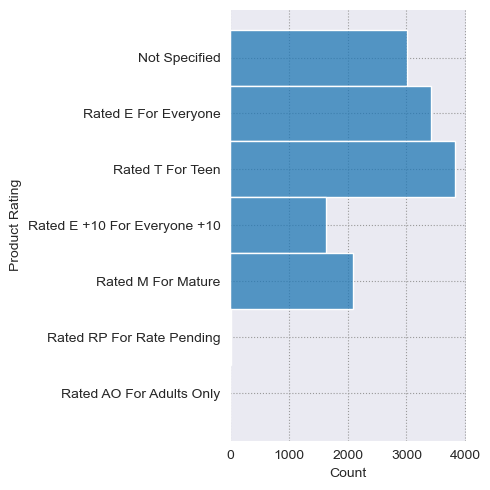
\includegraphics[width=0.5\linewidth]{Module_4_BigData//Proyecto//Propuestas//Imagenes/dataset1_ProductRating_histogram.png}
        \caption{Histograma Product Rating}
        \label{fig:hist_product_rating}
    \end{figure}

    \begin{figure}[hbtp!]
        \centering
        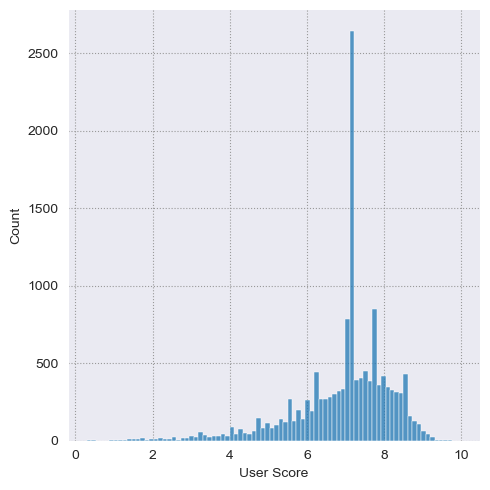
\includegraphics[width=0.5\linewidth]{Module_4_BigData//Proyecto//Propuestas//Imagenes/dataset1_UserScore_histogram.png}
        \caption{Histograma User Score}
        \label{fig:hist_user_score}
    \end{figure}

    Aunque se puede notar que en \ref{fig:hist_product_rating} hay dos categorías que no tiene datos, se ve una distribución saludable entre el resto. Por otro lado, se puede apreciar un desbalance con uno de los ratings en \ref{fig:hist_user_score}. Este desbalanceo se debe al reemplazo que se hizo anteriormente de los NaN, ya que este atributo contaba con muchos de ellos. A este punto, como este set de datos se piensa utilizar con información adicional del próximo conjunto de datos, no hay razón para lidiar con este problema en este momento.


\subsubsection{Segundo set: Video Game Sales 2024}
URL: \url{https://www.kaggle.com/datasets/asaniczka/video-game-sales-2024}\\
Este es el conjunto de datos principal, ya que cuenta con la información de las ventas actualizada hasta lo que se lleva de este año 2024. Cuenta con información de más de 64 mil video juegos. Los atributos en este set de datos son los siguientes:
    \begin{enumerate}
        \item \textit{img:} Imagen de la portada del video juego.
        \item \textit{title:} Nombre del video juego. \textbf{Esta va a ser la llave a utilizar para poder unir los dos set de datos.}
        \item \textit{console:} La plataforma donde se corre el video juego.
        \item \textit{genre:} El tipo de juego, ejemplos: acción, deportes, estrategia, otros.
        \item \textit{publisher:} Editor del video juego.
        \item \textit{developer:} Desarrollador del video juego.
        \item \textit{critic\_score:} Puntaje de la crítica.
        \item \textit{total\_sales:} Ventas totales a nivel mundial. \textbf{De los datos de este atributo se va a generar el objetivo predictivo.}
        \item \textit{na\_sales:} Ventas totales en Japón.
        \item \textit{jp\_sales:} Ventas totales en Estados Unidos.
        \item \textit{pal\_sales:} Ventas totales en Europa y África.
        \item \textit{other\_sales:} Ventas totales en otras regiones de menor volumen.
        \item \textit{release\_date:} Fecha del lanzamiento del video juego.
        \item \textit{last\_update:} Fecha de la última actualización de los datos.
    \end{enumerate}

\subsubsection{Calidad de datos:}
De forma similar con el set de datos anterior, empieza con entender la cantidad de valores NaN presentes en el conjunto de datos. Los resultados se tabulan a continuación:
    
    \begin{table}[hbtp!]
        \centering
        \begin{tabular}{|c|c|}
            \hline
            \textbf{Atributo} & \textbf{Conteo de NaN}\\
            \hline
            img & 0\\
            \hline
            title & 0\\
            \hline
            console & 0\\
            \hline
            genre & 0\\
            \hline
            publisher & 0\\
            \hline
            developer & 17\\
            \hline
            critic\_score & 57338\\
            \hline
            total\_sales & 45094\\
            \hline
            na\_sales & 51379\\
            \hline
            jp\_sales & 57290\\
            \hline
            pal\_sales & 51192\\
            \hline
            other\_sales & 48888\\
            \hline
            release\_date & 7051\\
            \hline
            last\_update & 46137\\
            \hline
        \end{tabular}
        \caption{Conteo de valores NaN en el set de datos Video Game Sales 2024}
        \label{tab:conteo_nan_info_videojuegos_ventas}
    \end{table}

    Aunque inicialmente se tenían mas de 64 mil instancias, el hecho que 45094 de ellas no tengan la información relacionada con las ventas totales indica que hay que descartar la mayoría de las instancias. No obstante, la cantidad restante es suficiente para el desarrollo de este proyecto.

    Con base a esto, se toman las siguientes decisiones para limpiar los datos: Primero, se eliminan los siguientes atributos:
    \begin{enumerate}
        \item img: No se necesita la imagen de la portada para este análisis.
        \item Todos los relacionados con ventas que no sea total\_sales: Dado que se quiere vender a nivel mundial, la información regional se descarta dando como prioridad la global.
        \item critic\_score: Es una práctica muy común que se pague por las buenas revisiones de los medios de la crítica, por lo tanto, este atributo podría introducir este ruido en el estudio.
        \item release\_date: Información presente en el set de datos anterior.
        \item last\_update: Información que no es relevante en este estudio.
        \item developer: Se descarta por la misma razón mencionada anteriormente. 
    \end{enumerate}

    Luego de esto, de desechan todas las instancias con NaN, lo que deja un total de 18922 instancias con 5 atributos. Es importante mencionar en este punto que, aunque este set de datos se queda con 5 atributos y el anterior con 6, algunos de estos atributos categóricos como console (39), publisher (733 en este último set de datos) y genres (19 en este último set de datos) contienen mucho valores distintos, lo que da pie a un estudio con más de 800 atributos.

\subsubsection{Análisis del segundo set de datos:}
Haciendo un enfoque en las ventas, veamos como se ven para generar la clase objetivo:

    \begin{figure}[hbtp!]
        \centering
        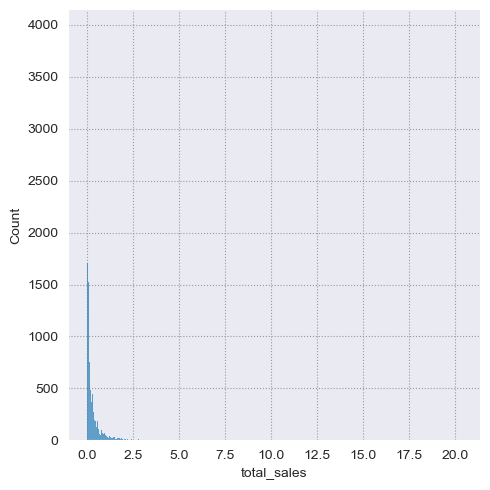
\includegraphics[width=0.5\linewidth]{Module_4_BigData//Proyecto//Propuestas//Imagenes/dataset2_totalVentasCompleto_histogram.png}
        \caption{Total de Ventas Globales}
        \label{fig:total_ventas_globales}
    \end{figure}

    En el histograma \ref{fig:total_ventas_globales} se aprecia que muy pocos video juegos que han vendido cantidades exorbitantes de unidades (por ejemplo, GTA 5 ha vendido mas de 20 millones de unidades). Estos outliers causan que se pierda visibilidad del punto de interés, las cuales son 100 mil copias. Por lo tanto, si se ignoran los video juegos que vendan más de 1 millón de copias, se observa lo siguiente:\newpage

    \begin{figure}[hbtp!]
        \centering
        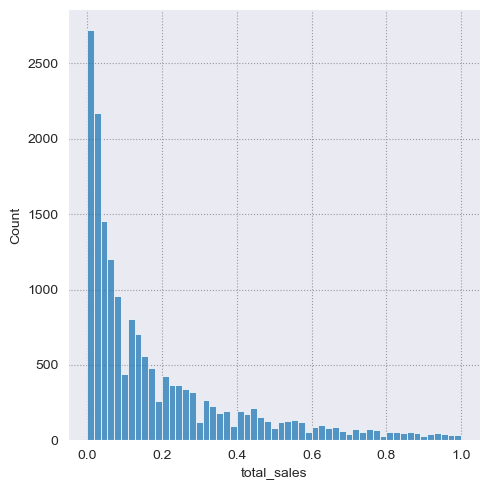
\includegraphics[width=0.5\linewidth]{Module_4_BigData//Proyecto//Propuestas//Imagenes/dataset2_totalVentas_menos1M_histogram.png}
        \caption{Ventas globales menores o iguales a 1 millón de copias}
        \label{fig:total_ventas_1M}
    \end{figure}

    Ahora los datos siguen, de forma muy fiel, una función de densidad exponencial. Se podría pensar que hay un problema de balanceo de datos, pero si se hace un corte entre todos los juegos que no han vendido mas de 100 mil copias contra los que sí lograron esa meta, se aprecia lo siguiente:

    \begin{figure}[hbtp!]
        \centering
        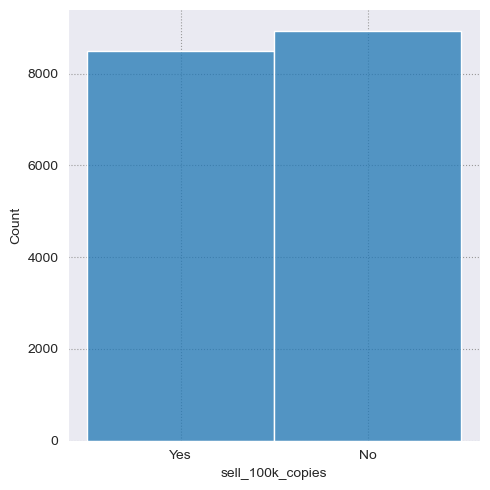
\includegraphics[width=0.5\linewidth]{Module_4_BigData//Proyecto//Propuestas//Imagenes/dataset2_totalVentas_categorizado_histogram.png}
        \caption{Total de ventas separado por juegos que vendieron m\'{a}s de 100 mil copias o no}
        \label{fig:total_ventas_categorizado}
    \end{figure}

    De esta forma, podemos ver en \ref{fig:total_ventas_categorizado} que la clase objetivo esta, prácticamente, perfectamente balanceada en este set de datos. \textbf{Este es el objetivo predictivo de esta propuesta.}
    
    Para concluir este análisis de datos, verificamos que no hayan problemas de balanceo entre otros atributos de interés:\newpage

    \begin{figure}[hbtp!]
        \centering
        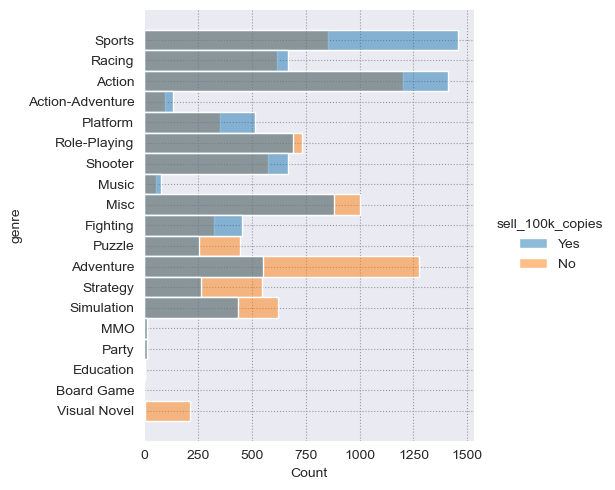
\includegraphics[width=0.5\linewidth]{Module_4_BigData//Proyecto//Propuestas//Imagenes/dataset2_genre_histogram.png}
        \caption{Histograma de los tipos de juegos, tomando en cuenta si vendieron 100 mil copias o no}
        \label{fig:hist_genre}
    \end{figure}

    Aunque en \ref{fig:hist_genre} se pueden ver 4 categorías predominantes, hay una buena distribución de datos entre varios tipos de video juegos.

    \begin{figure}[hbtp!]
        \centering
        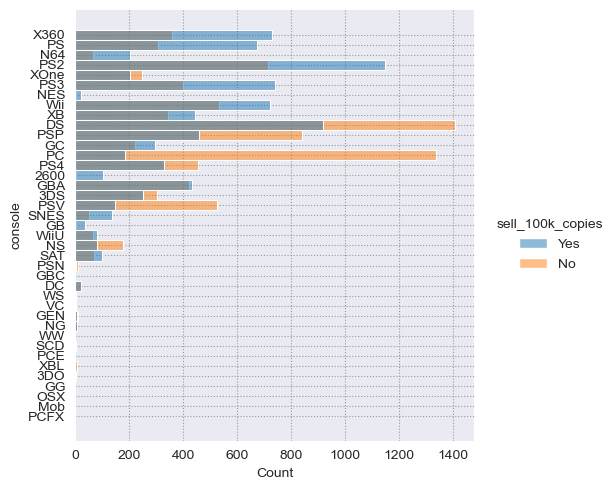
\includegraphics[width=0.5\linewidth]{Module_4_BigData//Proyecto//Propuestas//Imagenes/dataset2_consolas_histogram.png}
        \caption{Histograma de las consolas, tomando en cuenta si vendieron 100 mil copias o no}
        \label{fig:hist_consoles}
    \end{figure}

    Hay muchas consolas en \ref{fig:hist_consoles} en las cuales se observa que los juegos no son jugados, pero en las más populares se observa una distribución que no sugiere un problema de balanceo.

\subsubsection{Conclusión de la primera propuesta:}
Este es un problema de categorización binaria que presenta un reto interesante, dado que se tiene un objetivo predictivo balanceado, pero a la vez se cuenta con muchos datos categóricos que presentar retos importantes a la hora de modelar.



\subsection{Segunda propuesta: Desarrollar un animé que la gente vea por completo}
\subsubsection{Problema a resolver}
El animé tiene su origen en Japón a inicios del siglo 20. Desde ese momento, la popularidad de dicho arte ha ido en aumento, y gracias a una exposición más global a partir del acceso a plataformas de streaming que cuenta con este contenido. En 2023, el animé reportó un mercado de mas de \$32 mil millones de dolares, y por su tendencia en popularidad, se calcula que superará los \$70 mil millones para 2032 (\url{https://www.grandviewresearch.com/industry-analysis/anime-market}).\\

Un estudio de animación en Japón esta interesado en entrar en el mercado, pero en un ambiente tan competitivo, la cantidad de animés es tal que los servicios de streaming están tomando la iniciativa de dar un bono económico al estudio que cree animés que sean completados (ya sea en su totalidad o cada temporada, es decir, que lo lleven al día) dado que quieren mantener una concurrencia de usuarios en sus plataformas.

\subsubsection{Solución propuesta}
Hacer un estudio de mercado para entender los factores básicos que hacen que los usuarios terminen o lleven al día un animé particular. Por lo tanto, se plantea hacer el análisis por medio de un software con aprendizaje automático que sea capaz de predecir si un animé va a ser completado o no.

\subsubsection{Fuentes de datos}
Para hacer este estudio de mercado, se van a utilizar tres conjuntos de datos tomados de Kaggle. Los 3 set de datos vienen del URL: \url{https://www.kaggle.com/datasets/azathoth42/myanimelist}. A pesar de provenir del mismo lugar, los 3 dataset se manejan de forma independiente.\\

Para este problema en particular, se van a usar los CSV que ya tienen un primer filtro (tiene el término \textit{\_filtered)}. A pesar de estar filtrados, hay una cantidad muy grande de datos: Uno de estos cuenta con más de 32 millones de instancias, por lo tanto, para efectos de este trabajo, ese CSV va a ser reducido (más detalles adelante). El autor de este post en Kaggle menciona que estos datos provienen MyAnimeList.net, el cual es solo uno de muchas opciones de streaming hoy en dia, asi que este estudio NO cubre otros servicios de streaming importantes como lo son Netflix o Crunchyroll.

\subsubsection{Primer set: anime\_filtered.csv}
De entrada, este set de datos cuenta con 14474 instancias y 31 atributos distintos. Este número de atributos es manejable, pero muchos de ellos no aportan información valiosa. Por lo tanto, el primer paso es eliminar 19 de ellos.

\subsubsection{Calidad de datos:}
A continuación se listan y la razón por la cual se decidió eliminar del estudio:
\begin{enumerate}
    \item \textit{title\_english:} Esta información es redundante con otro atributo llamado "title".
    \item \textit{title\_japanese:} Esta información es redundante con otro atributo llamado "title", además de que no se quiere lidiar con caracteres en japones.
    \item \textit{title\_synonyms:} Esta información es redundante con otro atributo llamado "title".
    \item \textit{favorites:} Este atributo es redundante con respecto a la variable objetivo, ya que un usuario que tenga un animé en su lista de favoritos muy probablemente lo va a completar de ver.
    \item \textit{image\_url:} Es la imagen de la portada del animé, lo cual no es relevante para el estudio.
    \item \textit{broadcast:} Es la fecha en que se transmite el animé, ya esa en televisión japonesa o bien cuando sale un capitulo nuevo en el servicio de streaming. Este atributo esta sujeto a cambios continuos, por lo tanto, se volvería una variable difícil de estudiar.
    \item \textit{airing:} Indica si el animé esta en proceso de producción o no (si esta terminado o esta en curso). Este atributo es irrelevante dado que no es importante si está en producción o no, si no si los usuarios lo llevan al día o no.
    \item \textit{aired\_string:} Se descarta por la misma razón anterior.
    \item \textit{aired:} Se descarta por la misma razón anterior.
    \item \textit{scored\_by:} Este atributo indica quien le de dio una calificación al animé, lo cual es redundante con el usuario en sí.
    \item \textit{background:} Un poco mas de información del anime en si, pero sin ser relevante para el estudio o ser información que ya esta contenida en otro atributo.
    \item \textit{premiered:} Momento cuando el animé fue lanzado. De igual forma que con airing, lo importante es saber si fue completado o no, no cuando fue lanzando en sí.
    \item \textit{related:} Indica que otros animé son parecidos. Ya que se cuenta con una lista tan extensa de animé, no es necesario analizar esta relación.
    \item \textit{members:} Es el numero de usuarios que son miembros del animé. No queda claro a que se refiere este atributo, pero otro llamado favorite es semejante y da mejor información que éste.
    \item \textit{licensor:} Es el nombre de quien licencia la producción. Esta información es difícil de conseguir, por lo que alrededor del 77\% de este atributo tiene valores NaN, por lo que se decide descartarlo de entrada para no perder muchos de los datos.
    \item \textit{opening\_theme:} Es la canción que suena durante la introducción de cada capitulo, lo cual no es relevante para el estudio actual.
    \item \textit{ending\_theme:} Similar al anterior, es la canción que suena al final de cada capitulo. Se descarta por la misma razón anterior.
    \item \textit{studio:} Es el estudio quien desarrolla el animé. Similar a la propuesta anterior, es atributo no es de interés por parte del cliente dado que no quieren compararse contra las capacidad productivas de los competidores directos.
    \item \textit{rank:} Es el rango que tiene el animé, lo cual es redundante con la popularidad del mismo, por eso se descarta.
\end{enumerate}

Después de este primer descarte de atributos, se quedan los siguientes 12:
\begin{enumerate}
    \item \textit{anime\_id:} Es el ID de cada animé de la lista. \textbf{Este atributo se va a usar como llave de unión con el set de datos principal}
    \item \textit{title:} Nombre del animé, en ingles.
    \item \textit{type:} Predominan dos: TV y OVA, pero este atributo cuenta con mas de 6000 diferentes tipos. Por ahora no se va a analizar en profundidad y se va a tener que hacer una agrupación, pero se hará después de la unión con los otros dos set de datos (fuera de alcance para esta propuesta).
    \item \textit{source:} Indica cual fue la fuente de la historia del animé: una novela, un manga, otros.
    \item \textit{episodes:} La cantidad de episodios que tiene el animé.
    \item \textit{status:} Indica si la producción fue concluida o no.
    \item \textit{duration:} Cuanta es la duración promedio por episodio.
    \item \textit{rating:} Es la categoría del animé, por ejemplo: apto para todo público, mayores de cierta edad, para adultos, etc.
    \item \textit{score:} Es la calificación promedio del animé.
    \item \textit{popularity:} Un indicador de qué tan popular es el animé.
    \item \textit{producer:} El productor del animé. Cabe la pena resaltar que una producción de una animé normalmente requiere de varios productores a la vez.
    \item \textit{genre:} El genero del anime. Este atributo tiene la complejidad que un animé puede tener varios géneros.
\end{enumerate}

Un analisis de NaN muestra que no hay mayor problema de esta índole (64 instancias en el atributo genre), por lo que las filas con NaN son descartadas.

\subsubsection{Análisis del primer set de datos:}
Después de este punto se hizo un análisis visual de los atributos, pero para efectos prácticos de esta propuesta, se muestran solo los resultados finales. Para mas detalle del estudio que se hizo, por favor referirse al Jupyter Notebook de la propuesta \#2.

Estos resultados finales son:

\begin{figure}[hbtp!]
    \centering
    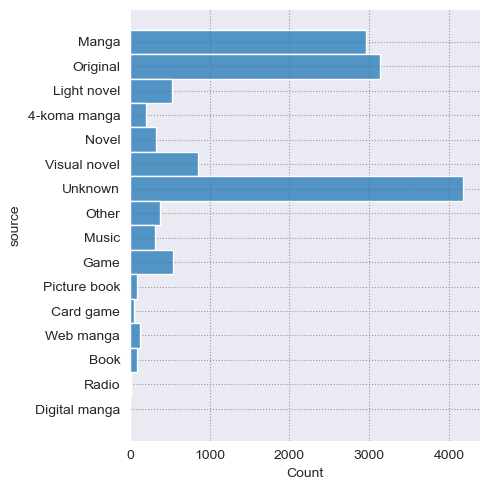
\includegraphics[width=0.5\linewidth]{Module_4_BigData//Proyecto//Propuestas//Imagenes/p2_dataset1_source_histogram.png}
    \caption{Histograma del atributo Source}
    \label{fig:hist_p2_dataset1_source}
\end{figure}

En la figura \ref{fig:hist_p2_dataset1_source} se nota que hay 3 principales sources para los animé: los mangas, historias originales o fuente desconocida. Para este atributo va a ser necesario hacer una estrategia de agrupamiento para lidiar con el desbalance. Dicho esto, esa estrategia no sera ejecutada en este momento de la propuesta.

\begin{figure}[hbtp!]
    \centering
    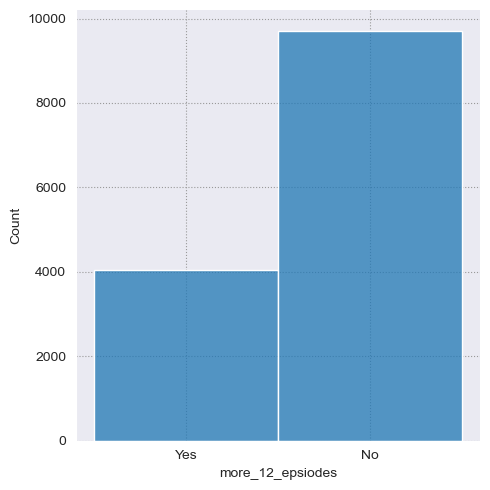
\includegraphics[width=0.5\linewidth]{Module_4_BigData//Proyecto//Propuestas//Imagenes/p2_dataset1_episodes_histogram.png}
    \caption{Histograma del atributo Episodes}
    \label{fig:hist_p2_dataset1_episodes}
\end{figure}

Para el caso del atributo nuevo llamado more\_12\_episodes que fue creado a partir de episodes, la figura \ref{fig:hist_p2_dataset1_episodes} muestra un problema de desbalance en la cantidad de animes que tienen 12 o menos episodios. Como este set de datos es de soporte para el set de datos principal, todavía no se va a lidiar con este problema.

\begin{figure}[hbtp!]
    \centering
    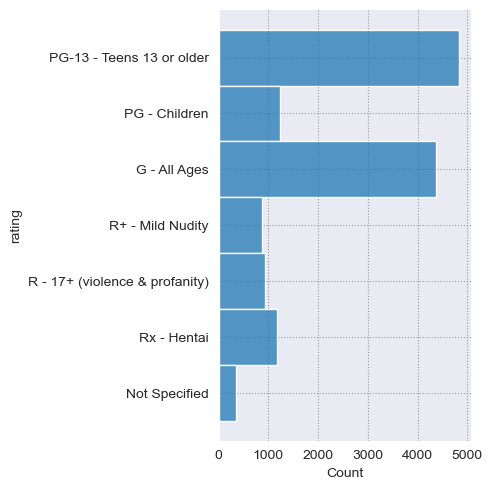
\includegraphics[width=0.5\linewidth]{Module_4_BigData//Proyecto//Propuestas//Imagenes/p2_dataset1_rating_histogram.png}
    \caption{Histograma del atributo Rating}
    \label{fig:hist_p2_dataset1_rating}
\end{figure}

Finalmente, en la figura \ref{fig:hist_p2_dataset1_rating} se nota otro problema de desbalanceo con los datos. En este caso, se podría hacer una agrupación para evitar este problema y tener solo 3 categorías, pero para efectos de la propuesta, esto todavía no se va a realizar.


\subsubsection{Segundo set: animelist\_filtered\_by\_anime.csv}
Este es el \textbf{set de datos principal} porque relaciona tanto los usuarios como el animé que vieron, y en cual estado lo tienen. Este CSV se creo a partir del que cuenta con mas de 23 millones de instancias. El set de datos cuenta con mas de 14 mil instancias y tiene 11 atributos, donde la mayoría están con valores de NaN o en cero, por lo que fueron descartados de entrada. Estos son: my\_start\_date, my\_finish\_date, my\_rewatching, my\_rewatching\_ep, my\_last\_updated y my\_tags.\\

Los atributos que quedan son los siguientes:
\begin{enumerate}
    \item \textit{username:} Este el nombre de usuario del servicio. \textbf{Esta es la llave de conexión el tercer ser de datos (por analizar más adelante)}
    \item \textit{anime\_id:} ID del anime. \textbf{Esta es la llave de conexión con el primer set de datos (ya analizado a este punto)}.
    \item \textit{my\_watched\_episodes:} La cantidad de episodios visto por el usuario del animé en cuestión.
    \item \textit{my\_score:} La calificación que el usuario le dio el animé.
    \item \textit{my\_status:} Indica el estado del animé con respecto al usuario. Este atributo tiene 5 categorias: 1 = watching, 2 = completed, 3 = on hold, 4 = dropped y 6 = plan to watch. \textbf{De este atributo se va a crear el objetivo predictivo de esta propuesta.}
\end{enumerate}

\subsubsection{Calidad de datos:}
En este punto, no es necesario trabajar en la calidad de los datos. Al eliminar las columnas sin información, el 100\% de los NaN se eliminar y el resto del set de datos es válido.

\subsubsection{Análisis del segundo set de datos:}
Para este set de datos se va a analizar solamente el objetivo predictivo. De forma individual, los estados se ven de la siguiente forma:

\begin{figure}[hbtp!]
    \centering
    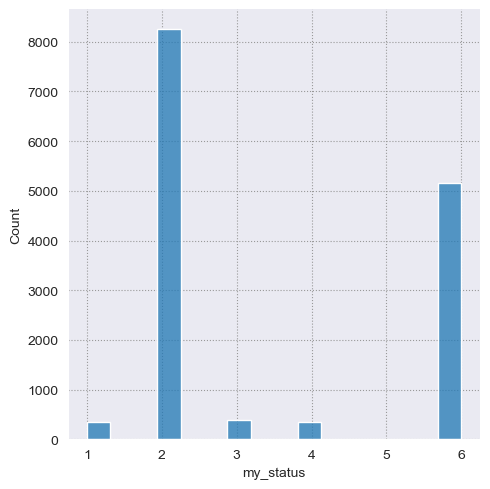
\includegraphics[width=0.5\linewidth]{Module_4_BigData//Proyecto//Propuestas//Imagenes/p2_dataset2_status_histogram.png}
    \caption{Histograma del atributo Status (individual)}
    \label{fig:hist_status_individual}
\end{figure}

De la figura \ref{fig:hist_status_individual} se concluye que hay dos estados que predominan sobre el resto: Completados (2) y Por Ver (6). El resto de los estados son bastante menores. Para crear el objetivo predictivo hay que agrupas todas la categorías juntos excepto la 2, para poder  tener idea de como se ve la condición de completado contra el resto. Los resultados son los siguientes:

\begin{figure}[hbtp!]
    \centering
    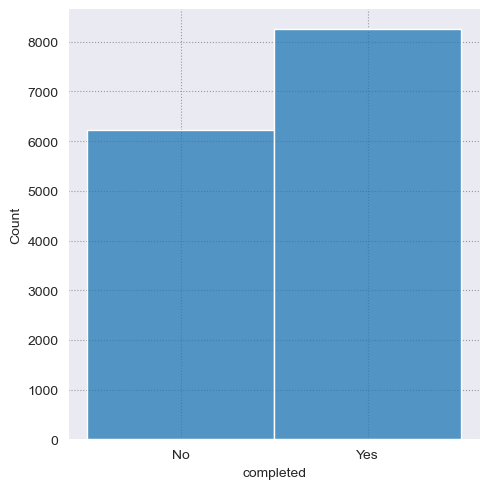
\includegraphics[width=0.5\linewidth]{Module_4_BigData//Proyecto//Propuestas//Imagenes/p2_dataset2_status_grouped_histogram.png}
    \caption{Histograma del atributo Status (agrupado)}
    \label{fig:hist_status_grouped}
\end{figure}

Visto de esta forma, la figura \ref{fig:hist_status_grouped} evidencia que el objetivo predictivo tiene un balance aceptable para poder hacer un categorización.

\subsubsection{Tercer set: users\_filtered.csv}
Este último se de datos es la información de los usuarios, que cuenta con algunos atributos demográficos, y que tiene como finalidad dar mas atributos segundo set de datos.

Aquí se cuentan con mas de 116 mil instancias con 17 atributos. A continuación la lista de todos los atributos y en que consiste cada uno y si fue descartado o no:
\begin{enumerate}
    \item \textit{username:} Nombre del usuario. \textbf{Esta es la llave de unión con el segundo set de datos.}
    \item \textit{user\_id:} ID del usuario. Se descarte porque es redundante con el nombre.
    \item \textit{user\_watching:} Cantidad de animes que el usuario esta viendo actualmente. Esta cantidad no representa ninguna información importante, además de ser cubierto por el segundo set de datos, por lo tanto, se descarta.
    \item \textit{user\_completed:} Cantidad de animes que el usuario ha completado. Esta cantidad no representa ninguna información importante, además de ser cubierto por el segundo set de datos, por lo tanto, se descarta.
    \item \textit{user\_onhold:} Cantidad de animes que el usuario tiene en pausa. Esta cantidad no representa ninguna información importante, además de ser cubierto por el segundo set de datos, por lo tanto, se descarta.
    \item \textit{user\_dropped:} Cantidad de animes que el usuario no va a continuar viendo. Esta cantidad no representa ninguna información importante, además de ser cubierto por el segundo set de datos, por lo tanto, se descarta.
    \item \textit{user\_plantowatch:} Cantidad de animes que el usuario planea ver eventualmente. Esta cantidad no representa ninguna información importante, además de ser cubierto por el segundo set de datos, por lo tanto, se descarta.
    \item \textit{user\_days\_spent\_watching:} Promedio de días que el usuario invierte viendo animé.
    \item \textit{gender:} Genero del usuario.
    \item \textit{location:} Localidad del usuario.
    \item \textit{birth\_date:} Fecha de nacimiento del usuario.
    \item \textit{access\_rank:} No se provee información, por lo tanto, se descarta.
    \item \textit{join\_date:} Fecha en la que el usuario creó su cuenta en el servicio de streaming.
    \item \textit{last\_online:} Última fecha registrada del usuario usando el servicio. Esta información no es relevante en el estudio y se descarta.
    \item \textit{stats\_mean\_score:} Promedio de calificación que da el usuario.
    \item \textit{stats\_rewatched:} No queda muy claro de que se trata este atributo, se decide descartar.
    \item \textit{stats\_episodes:} No queda muy claro de que se trata este atributo, se decide descartar.
\end{enumerate}

\subsubsection{Calidad de datos:}
Al igual que con el set de datos anterior, no es necesario trabajar en la calidad de los datos dado que la cantidad de NaN es poca (6 en el peor de los casos), por lo que se decide eliminar esas instancias.

\subsubsection{Análisis del tercer set de datos:}
Este set de datos cuenta con casi 43 mil locaciones diferentes entre todos los usuarios, por lo tanto, no se puede mostrar un análisis visual de este atributo.

Veamos entonces los histogramas del género del usuario y su media de calificación:\newpage

\begin{figure}[hbtp!]
    \centering
    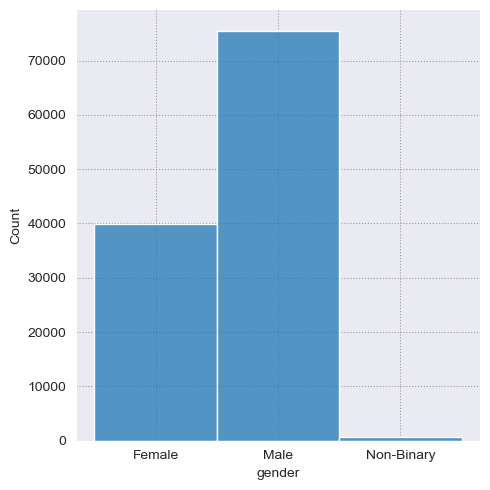
\includegraphics[width=0.5\linewidth]{Module_4_BigData//Proyecto//Propuestas//Imagenes/p2_dataset3_user_gender_histogram.png}
    \caption{Histograma del género de los usuarios}
    \label{fig:hist_p2_dataset3_gender}
\end{figure}

Analizando los géneros, la figura \ref{fig:hist_p2_dataset3_gender} muestra una clara tendencia problemas de desbalanceo entre hombres y mujeres, y de estos dos contra No Binario. Como este es un set de datos de soporte, ya una vez unificado con los demás se podría evaluar esta condición de nuevo, dado que aquí hay 116 mil instancias pero en el set de datos principal solo se cuenta con mas de 14 mil, por lo tanto, este escenario podría cambiar.

\begin{figure}[hbtp!]
    \centering
    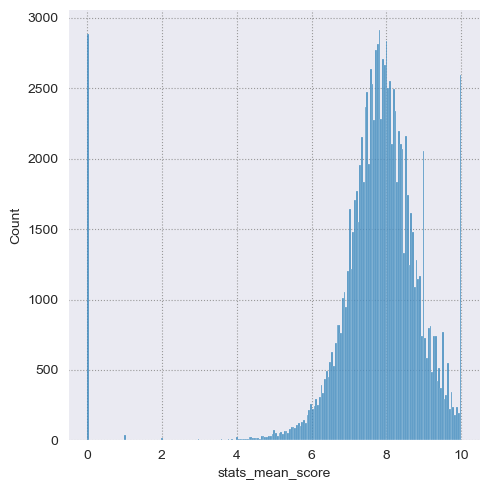
\includegraphics[width=0.5\linewidth]{Module_4_BigData//Proyecto//Propuestas//Imagenes/p2_dataset3_user_mean_score_histogram.png}
    \caption{Histograma del mean score por usuario}
    \label{fig:hist_p2_dataset3_mean_score}
\end{figure}

Y para concluir, la figura \ref{fig:hist_p2_dataset3_mean_score} muestra 3 condiciones interesantes: una distribución normal de las medias entre 4 y 10, pero con una fuerte presencia de 0 o de 10. Siguiendo una estrategia similar al atributo anterior, es necesario unificar los datos para tener una mejor idea del escenario que se tiene con este atributo.

\subsubsection{Conclusión de la segunda propuesta:}
Esta propuesta tiene un objetivo predictivo con un balance aceptable, y cuenta con el reto de unir 3 set de datos distintos y evaluar condiciones de desbalanceo junto con atributos que presentan combinaciones de categorías, lo cual es necesario desempacar para tener una buena idea de los géneros y los productores, que a la vez generaría una cantidad muy importante de atributos por considerar.

\end{document}